\chapter{阶梯波发生器的设计与仿真}%
\label{cha:阶梯波发生器的设计与仿真}

\section{实验目的}%
\label{sec:\arabic{chapter}实验目的}

\begin{enumerate}
	\item 设计一个能产生周期性阶梯波的电路,要求阶梯波周期在\SI{30}{\ms}左右,输出电压范围\SI{10}{\V},阶梯个数5个;(注意:电路中均采用模拟、真实器件,不可以选用计数器、555定时器、D/A转换器等数字器件,也不可选用虚拟器件。)对电路进行分段测试和调节,直至输出合适的阶梯波;
	\item 改变电路元器件参数,观察输出波形的变化,确定影响阶梯波电压范围和周期的元器件;
	\item 使用直流扫描分析(DCSweep)工具绘制结型场效应管的转移特性曲线,分析场效应管参数$ I_\mathrm{DSS} $对阶梯波影响的参数。
\end{enumerate}

\section{实验要求}%
\label{sec:\arabic{chapter}实验要求}

\begin{Exercise}
	给出阶梯波发生器实验原理图。
\end{Exercise}

\begin{Answer}
	阶梯波发生器实验原理图见图\ref{fig:阶梯波发生器电路图}。
\end{Answer}

\begin{Exercise}
	介绍电路的工作原理。
\end{Exercise}

\begin{Answer}
	工作原理见章节\ref{sub:\arabic{chapter}仿真结果}。
\end{Answer}

\begin{Exercise}
	给出电路的分段测试波形和最终输出的阶梯波,并回答以下问题:
	\begin{enumerate}
		\item 调节电路中哪些元器件值可以改变阶梯波的周期?
		\item 调节电路中哪些元器件值可以改变阶梯波的输出电压范围?
		\item 调节电路中哪些元器件值可以改变阶梯波的阶梯个数。
	\end{enumerate}
\end{Exercise}

\begin{Answer}
	分段测试波形见图\ref{fig:方波波形图}、\ref{fig:微分电路波形}、\ref{fig:限幅电路波形}、\ref{fig:积分电路波形}、\ref{fig:脉冲波形},最终输出的阶梯波见图\ref{fig:向上阶梯波形}。调节电路中元器件值见章节\ref{sub:\arabic{chapter}指标计算}。
\end{Answer}

\begin{Exercise}
	说明设计和调试过程中出现的问题与解决办法,以及改进和创新性方案。
\end{Exercise}

\begin{Answer}
	设计和调试过程中出现的问题与解决办法见章节\ref{sub:\arabic{chapter}误差分析},改进和创新性方案见章节\ref{ssub:向下阶梯波形}。
\end{Answer}

\section{实验步骤}%
\label{sec:\arabic{chapter}实验步骤}

\subsection{设计电路}%
\label{sub:\arabic{chapter}设计电路}

\begin{figure}[H]
	\centering
	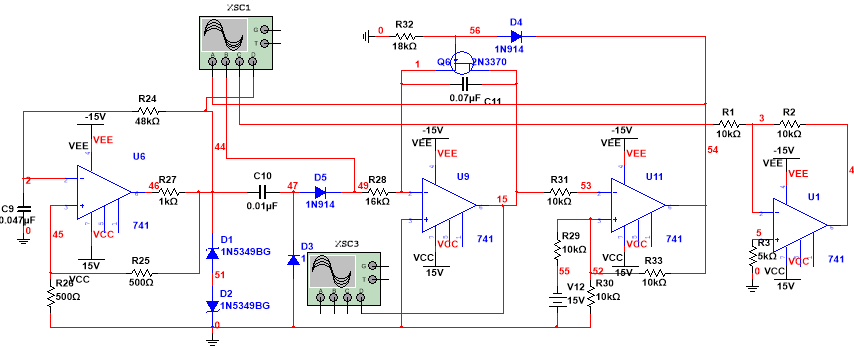
\includegraphics[width=0.8\linewidth]{4/JFET.png}
	\caption{阶梯波发生器电路图}
	\label{fig:阶梯波发生器电路图}
\end{figure}

\subsection{指标计算}%
\label{sub:\arabic{chapter}指标计算}

\begin{enumerate}
	\item 根据方波发生器的周期$ T = 2R_1C_1\ln(1 + 2\dfrac{R_2}{R_4}) $可得,改变$ R_4,C_1,R_1,R_2 $的值可以改变阶梯波的周期。
	\item 根据原理可知,输出电压范围和滞回比较器的门限电压有关。所以改变$ R_7,R_8 $可以改变输出电压。改变滞回比较器的直流电源值也会影响输出电压范围。
	\item 要改变阶梯波的阶梯个数:

		\begin{enumerate}
			\item 可以改变积分的高度,即改变微分电路和积分电路内部元器件参数。使得在一个周期中有更多或者更少的阶梯数;
			\item 改变迟滞比较器的的上下限的值。
		\end{enumerate}
\end{enumerate}

\subsection{仿真结果}%
\label{sub:\arabic{chapter}仿真结果}

\subsubsection{方波发生器}%
\label{ssub:方波发生器}

\begin{wrapfigure}{r}{0.6\linewidth}
	\centering
	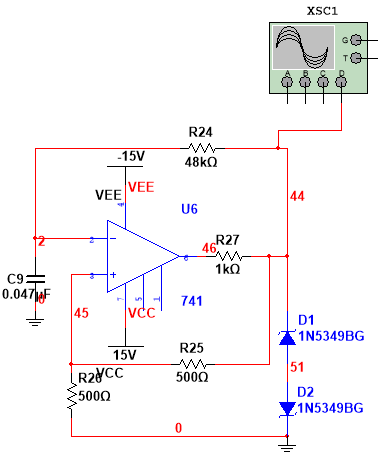
\includegraphics[width=\linewidth]{4/squareJFET.png}
	\caption{方波发生器}
	\label{fig:方波发生器}
\end{wrapfigure}

方波发生器是运放非线性运用,工作原理为当输入端为高电平时通过$ R_\mathrm{f}, C $电路放电直到电容两端电压达到翻转电压,此时运算放大器翻转,输出电压变为负值,此时通过$ R_\mathrm{f}C $电路充电直到翻转电压;方波发生器通过充放电在两种状态中循环切换,形成周期方波。

其中$ D_{1},D_{2} $为稳压管,导通电压\SI{10}{\V},配合$ R_{24} $实现输出电压限幅;

芯片同相输入端接$ R_{25}, R_{26} $,决定了翻转电压$ V_+ = \dfrac{R_{26}}{R_{25}+R_{26}}V_\mathrm{omax} $、$ V_- = \dfrac{R_{26}}{R_{25}+R_{26}}V_\mathrm{omin} $;

芯片反相输入端$ R_{24}, C_9 $组成充放电电路,时间常数为$ \dfrac{1}{R_\mathrm{f}C} $;

周期$ T = 2R_\mathrm{f}C\ln(1 + 2\dfrac{R_2}{R_3}) $为满足五个阶梯波周期为\SI{30}{\ms},因此方波周期为\SI{6}{\ms},构造$ R_{25}, R_{26} $为相同值,$ R_\mathrm{f} = \SI{48}{\kohm} $,$ C = \SI{0.047}{\mu\F} $,满足周期要求。

方波波形图如图\ref{fig:方波波形图}所示。

\begin{figure}[H]
	\centering
	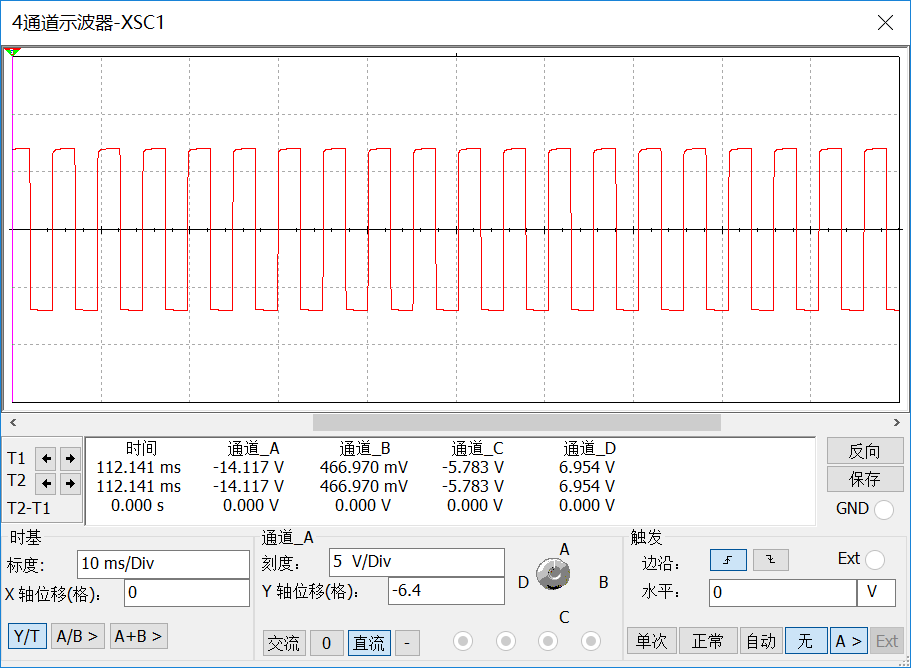
\includegraphics[width = 0.8\linewidth]{4/square.png}
	\caption{方波波形图}
	\label{fig:方波波形图}
\end{figure}

\newpage

\subsubsection{微分电路}%
\label{ssub:微分电路}

\begin{figure}[H]
	\centering
	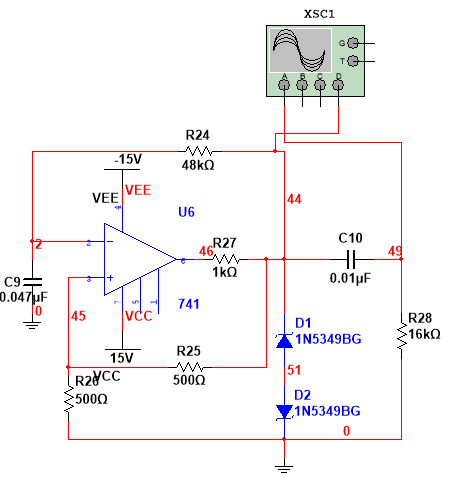
\includegraphics[width=.8\linewidth]{4/diffJFET.png}
	\caption{微分电路}
	\label{fig:微分电路}
\end{figure}

微分电路如图所示,主要是电容$ C_{10}, R_{28} $进行充放电,由于时间常数$ C_{10}R_{28} $比较小因此方波变成了尖脉冲形式,尖脉冲位置都在在方波突变位置。

微分电路波形如图\ref{fig:微分电路波形}所示。

\begin{figure}[H]
	\centering
	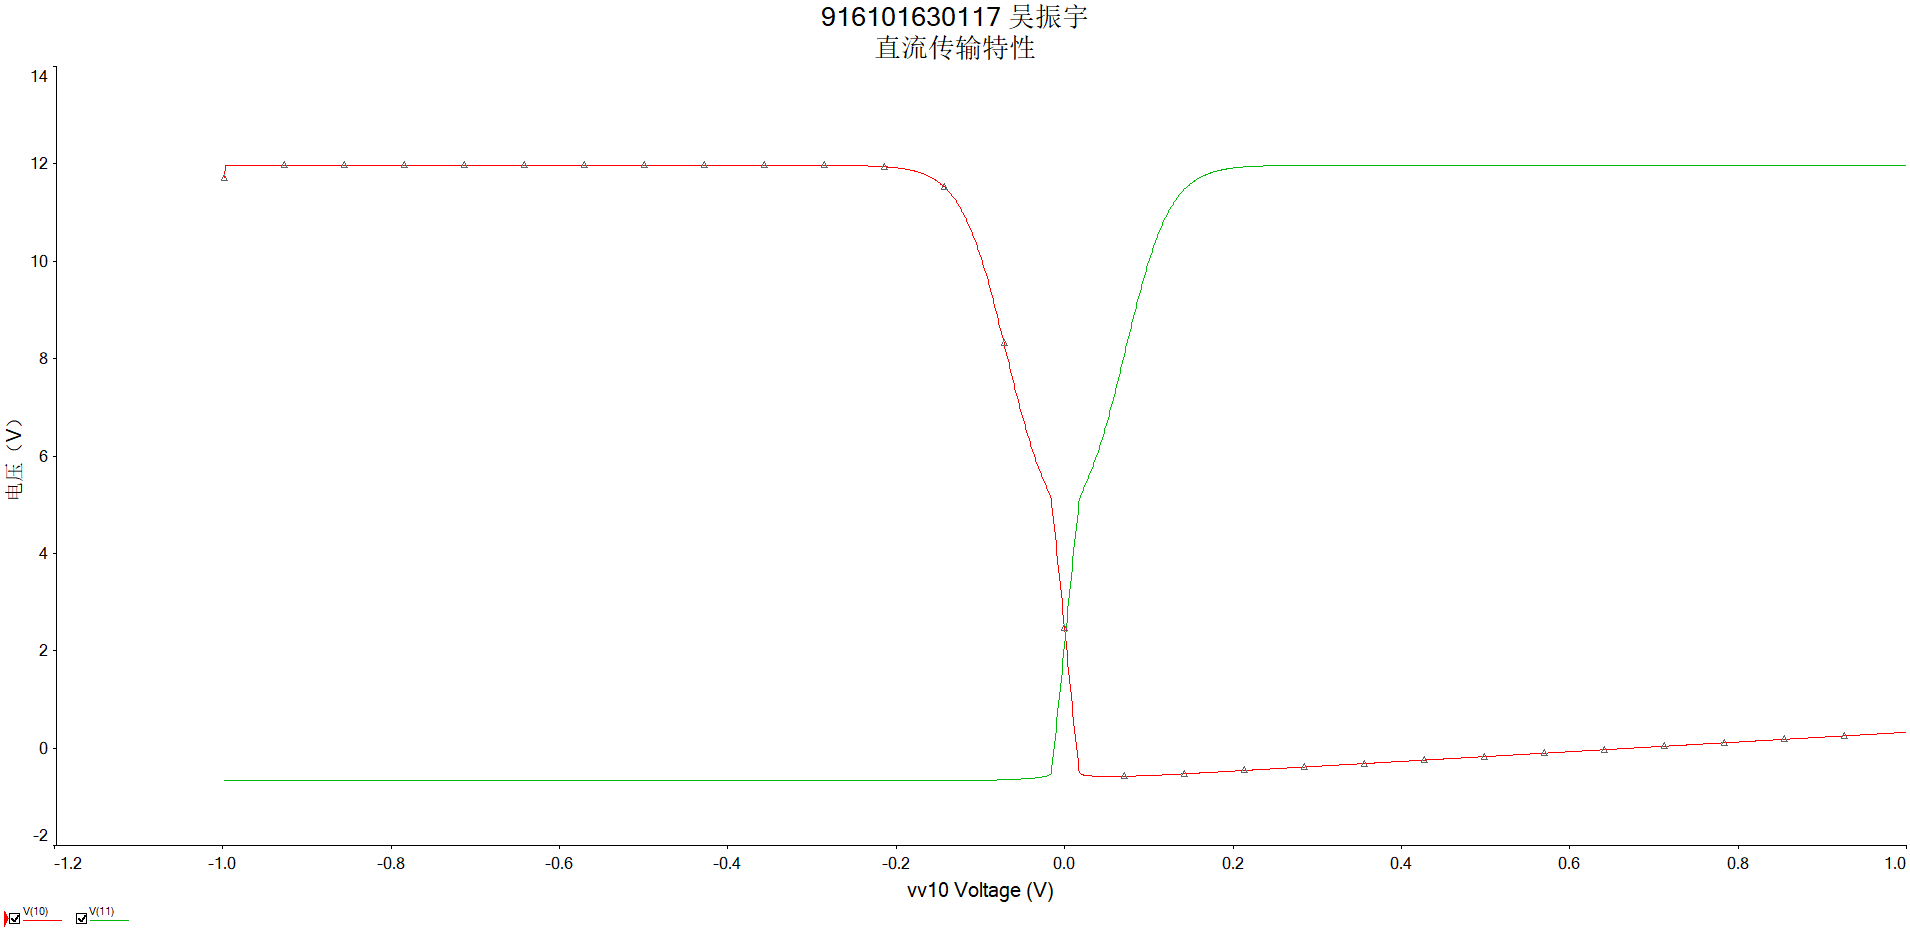
\includegraphics[width=0.8\linewidth]{4/diff.png}
	\caption{微分电路波形}
	\label{fig:微分电路波形}
\end{figure}

\subsubsection{限幅电路}%
\label{ssub:限幅电路}

\begin{figure}[H]
	\centering
	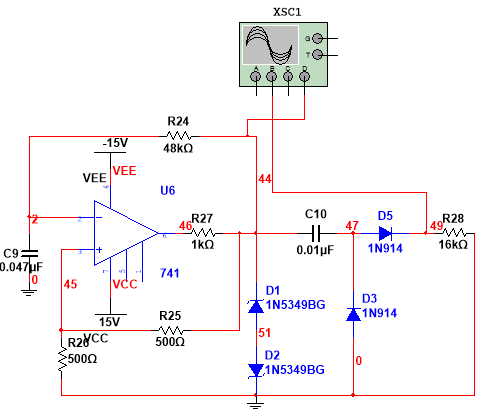
\includegraphics[width=0.8\linewidth]{4/limitJFET.png}
	\caption{限幅电路}
	\label{fig:限幅电路}
\end{figure}

限幅电路如图所示,主要是通过二极管$ D_3, D_5 $完成限幅功能。方波正周期时,$ D_5 $导通,$ C_{10}, R_{28} $构成微分电路形成正向尖脉冲,负周期时$ D_3 $导通、电容直接接地,不产生负周期尖脉冲。因此完成了限幅功能。

限幅波形如图\ref{fig:限幅电路波形}所示。

\begin{figure}[H]
	\centering
	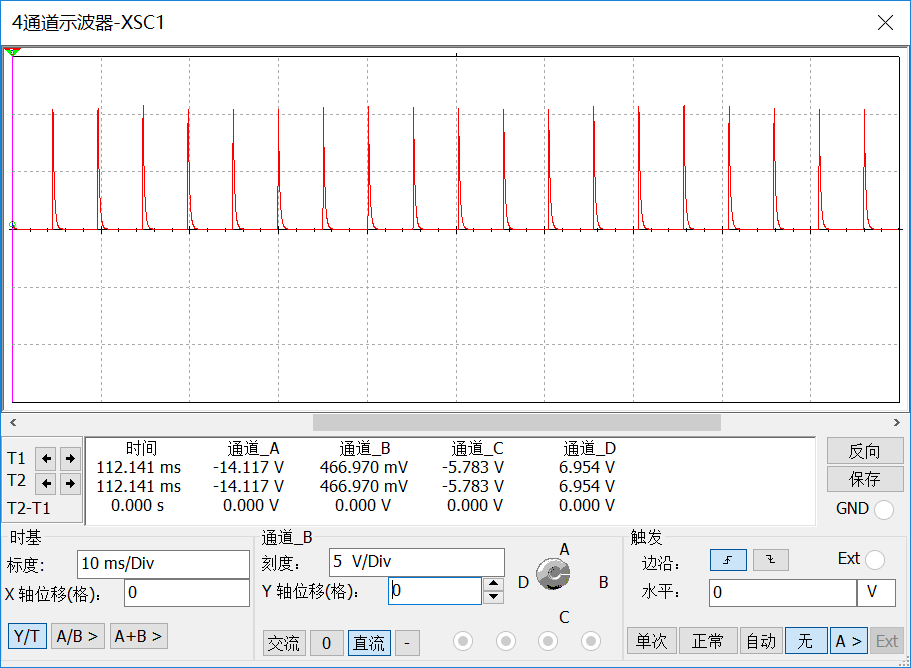
\includegraphics[width = 0.8\linewidth]{4/limit.png}
	\caption{限幅电路波形}
	\label{fig:限幅电路波形}
\end{figure}

\subsubsection{积分电路}%
\label{ssub:积分电路}

\begin{figure}[H]
	\centering
	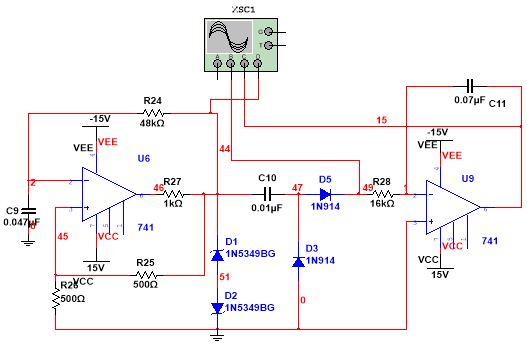
\includegraphics[width=0.8\linewidth]{4/integrateJFET.png}
	\caption{积分电路}
	\label{fig:积分电路}
\end{figure}

积分电路主要由$ R_{28}, C_{11} $以及运放组成。积分电路输入端是尖脉冲,因此积分时间很短,是积分输出波形几乎是发生突变、且在下一个尖脉冲到来之前输出端电压保持不变构成阶梯波的形式。

由于设计要求周期为\SI{}{\ms}级别,因此$ R_{28}C_{11} $单位为\SI{}{\ms}。

根据周期和峰值要求选用$ R_{28} = \SI{16}{\kohm}, C_3 = \SI{0.07}{\mu\F} $。

积分电路波形如图\ref{fig:积分电路波形}所示,上下限为电源电压\SI{15}{\V}左右。

\begin{figure}[H]
	\centering
	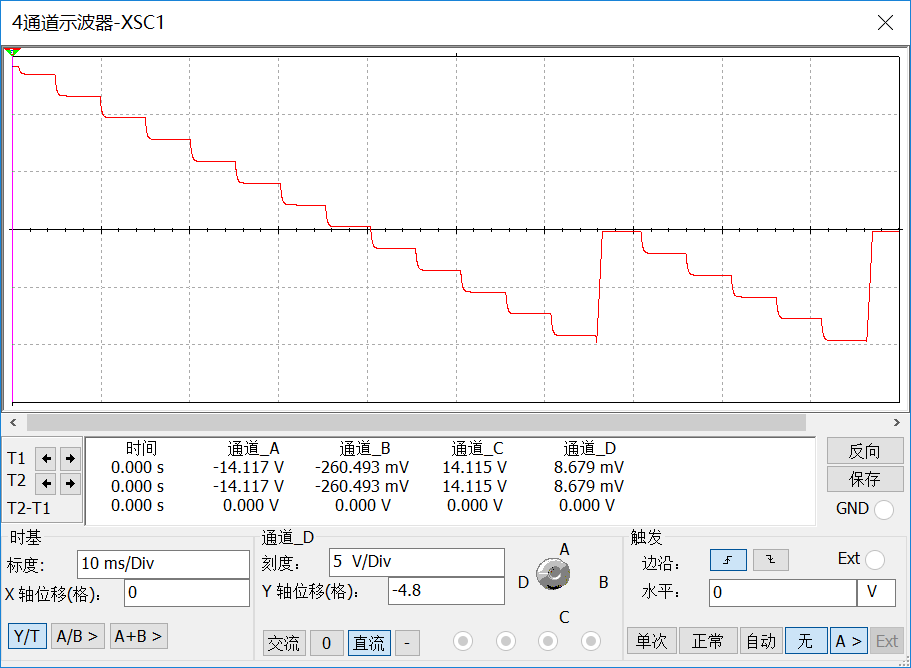
\includegraphics[width = 0.8\linewidth]{4/integrate.png}
	\caption{积分电路波形}
	\label{fig:积分电路波形}
\end{figure}

\subsubsection{比较器及电子开关电路}%
\label{ssub:比较器及电子开关电路}

\begin{figure}[H]
	\centering
	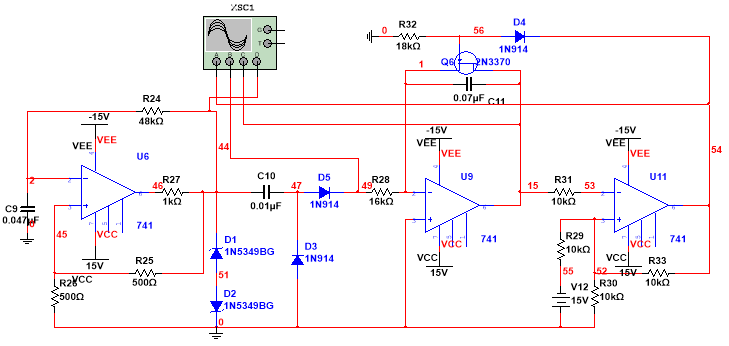
\includegraphics[width=\linewidth]{4/pulseJFET.png}
	\caption{比较器及电子开关电路}
	\label{fig:比较器及电子开关电路}
\end{figure}

比较器及电子开关电路如图\ref{fig:比较器及电子开关电路}所示。

其中比较器为迟滞比较器,主要由运放$ U_{11}, R_{31}, R_{29}, R_{30}, R_{33} $、参考电压$ V_{11} $组成。$ R_{31} $主要是限制输入电流保护运放;$ V_{12} $构成参考电压$ -V_\mathrm{R} $;通过调整$ R_{29}, R_{30}, R_{33} $能够调整门限电压。

电子开关电路由$ D_4 $、MOS管$ U_{11} $组成。当运放$ U_{11} $输出负值时电子开关关断、$ D_4 $不导通,输出回路对方波发生器无影响;当运放$ U_{11} $输出正值时电子开关导通、$ D_4 $也导通。

电路稳定时主要工作原理是反向输入端输入阶梯波,此时大于下门限电压,输出\SI{-15}{\V},此时$ D_4 $导通,场效应管栅极电压为负值,负电压使场效应管处于夹断状态,N沟道场效应管不能导通,同时$ D_4 $截止,比较器对方波发生器无影响;积分器输出电压不断降低,阶梯个数逐渐增加时,反相输入端到达下门限电压后比较器翻转输出\SI{+15}{\V},此时$ D_4 $截止,场效应管栅极电压变为0,场效应管导通,通过电容$ C11 $迅速放电,同时$ D_4 $变为导通,方波发生器输出负值,即比较器翻转时方波发生器输出负值使阶梯波起始波形相同。

由于设计要求5个阶梯波\SI{10}{\V}左右,因此上门限电压选为\SI{0}{\V},下门限电压选为\SI{-10}{\V},由于输出电压为\SI{+-15}{\V},因此选参考电压$ V_\mathrm{R} = \SI{-15}{\V} $,因此下门限电压等于$ \SI{-10}{\V} = \dfrac{V_\mathrm{omin} + V_\mathrm{R}}{3} $,上门限电压$ \SI{0}{\V} = \dfrac{V_\mathrm{omax} + V_\mathrm{R}}{3} $,因此$ R_{29}, R_{30}, R_{33} $均为\SI{10}{\kohm},$ R_{29}\parallel R_{30} $为\SI{5}{\kohm},分压为$ \dfrac{V_\mathrm{o}}{3} $,符合设计要求。

\begin{figure}[H]
	\centering
	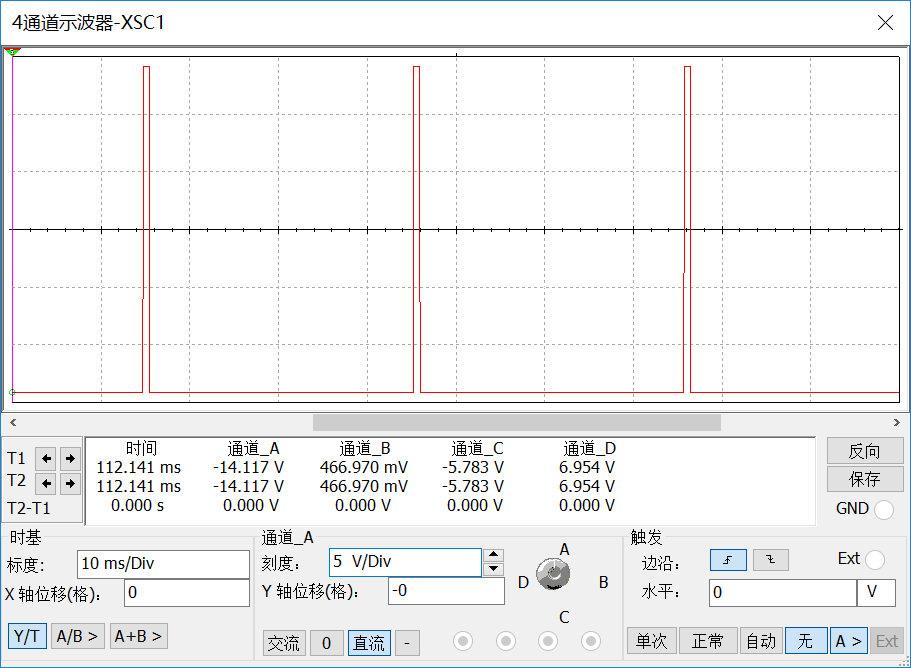
\includegraphics[width = 0.8\linewidth]{4/pulse.png}
	\caption{脉冲波形}
	\label{fig:脉冲波形}
\end{figure}

最终阶梯波形如图\ref{fig:向上阶梯波形}所示。符合设计要求,$ T = \SI{30}{\ms} $,输出电压幅值为\SI{10}{\V}左右。

\begin{figure}[H]
	\centering
	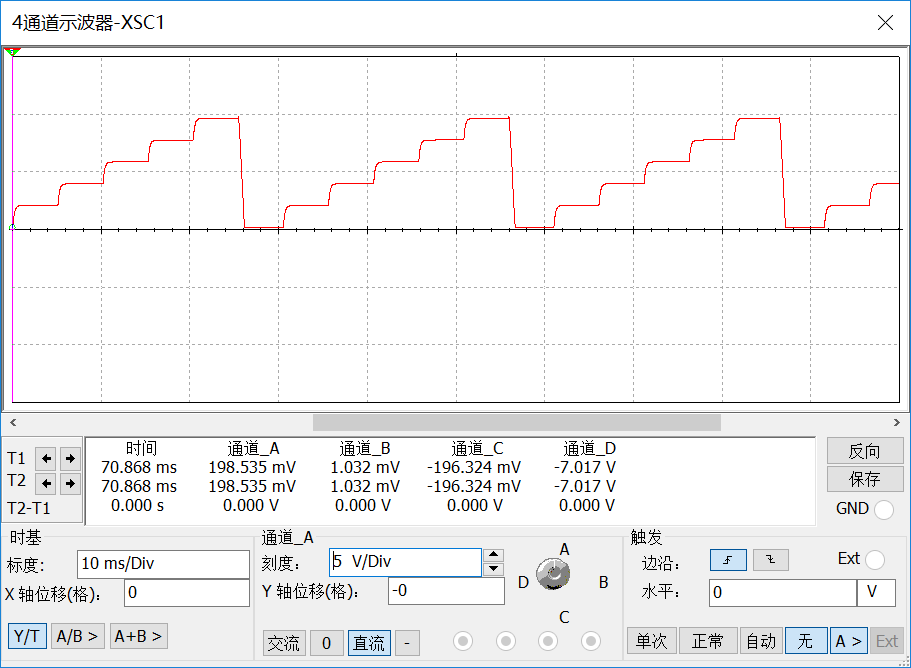
\includegraphics[width = 0.8\linewidth]{4/up.png}
	\caption{向上阶梯波形}
	\label{fig:向上阶梯波形}
\end{figure}

\subsubsection{向下阶梯波形}%
\label{ssub:向下阶梯波形}

如图\ref{fig:阶梯波发生器电路图},通过添加一个反相器可以得到向下阶梯波形。如图\ref{fig:向下阶梯波形}所示。

\begin{figure}[H]
	\centering
	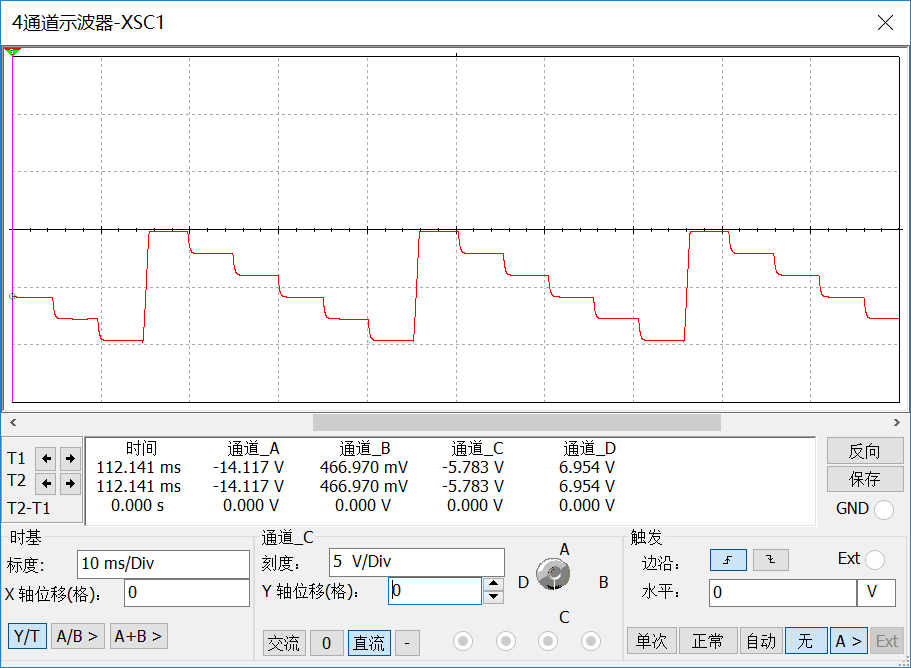
\includegraphics[width = 0.8\linewidth]{4/down.png}
	\caption{向下阶梯波形}
	\label{fig:向下阶梯波形}
\end{figure}

\subsubsection{三极管阶梯波发生器}%
\label{ssub:三极管阶梯波发生器}

\begin{figure}[H]
	\centering
	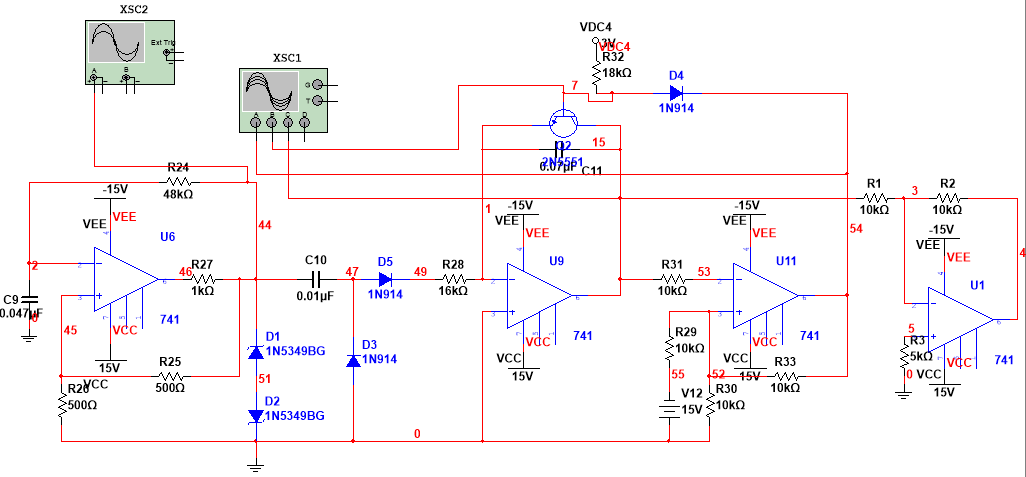
\includegraphics[width = \linewidth]{4/BJT.png}
	\caption{三极管阶梯波发生器}
	\label{fig:三极管阶梯波发生器}
\end{figure}

三极管阶梯波发生器电路图如图\ref{fig:三极管阶梯波发生器}所示。选用开关三极管替换
场效应管可以得到与原来阶梯波相近的波形。

\subsection{误差分析}%
\label{sub:\arabic{chapter}误差分析}

\begin{description}
	\item[阶梯波上升直线倾斜:]场效应管选择不当。
	\item[阶梯宽度不一致:]适当调节电阻大小,以重新满足周期要求。
	\item[毛刺:]门限电平未能控制好,调节电阻使门限电平尽可能接近\SI{10}{\V}。
\end{description}

\section{实验小结}%
\label{sec:\arabic{chapter}实验小结}

在这次实验中设计了一个具有一定功能的电路。先将一个项目细分为小的问题,再逐一解决。在这期间,查资料、计算、对相应的电路进行测验以检测其正确性。

这是通过Multisim进行设计仿真,对搭建实际电路有巨大的帮助作用。通过仿真软件,设计人员可以轻松的进行电路设计、参数调整。这对解决实际问题有着巨大的帮助。

